\documentclass{article}
\usepackage[utf8]{inputenc}
\usepackage{amsmath}
\usepackage{amsthm}
\usepackage{graphicx}
\graphicspath{{./images/}}
\usepackage[a4paper, margin=1in]{geometry}
\usepackage{float}
\usepackage{indentfirst}

\newtheorem{theorem}{Theorem}
\newtheorem{lemma}{Lemma}
\newtheorem{definition}{Definition}

\makeatletter
\newenvironment{shiftedflalign}{
	\start@align\tw@\st@rredfalse\m@ne
	\qquad\qquad
}{
	\endalign
}
\newenvironment{shiftedflalign*}{
	\start@align\tw@\st@rredtrue\m@ne
	\qquad\qquad
}{
	\endalign
}
\makeatother

\title{\textbf{\Large{Identifiability of the Causal Effect of $Infection$ on $Death$}}}
\author{\textbf{Rose Glavin} \smallskip \\ USF \smallskip \\ rose_glavin@hotmail.com}
\date{}

\begin{document}

\maketitle

\section{Task}

The qualitative knowledge of causal relationships in the domain is represented by a causal model shown in Fig. \ref{figure1}.
The treatment variable is $Infection$ and the outcome variable is $Death$.
We show that the causal effect $do(Infection = infection)$ on $Death$, written as $P_{Infection}\left(Death\right)$, is identifiable from a distribution over the observed variables $P\left(AHD,COPD,Death,Diabetes,HT,ICU,Infection\right)$.

\begin{figure}[H]
	\centering
	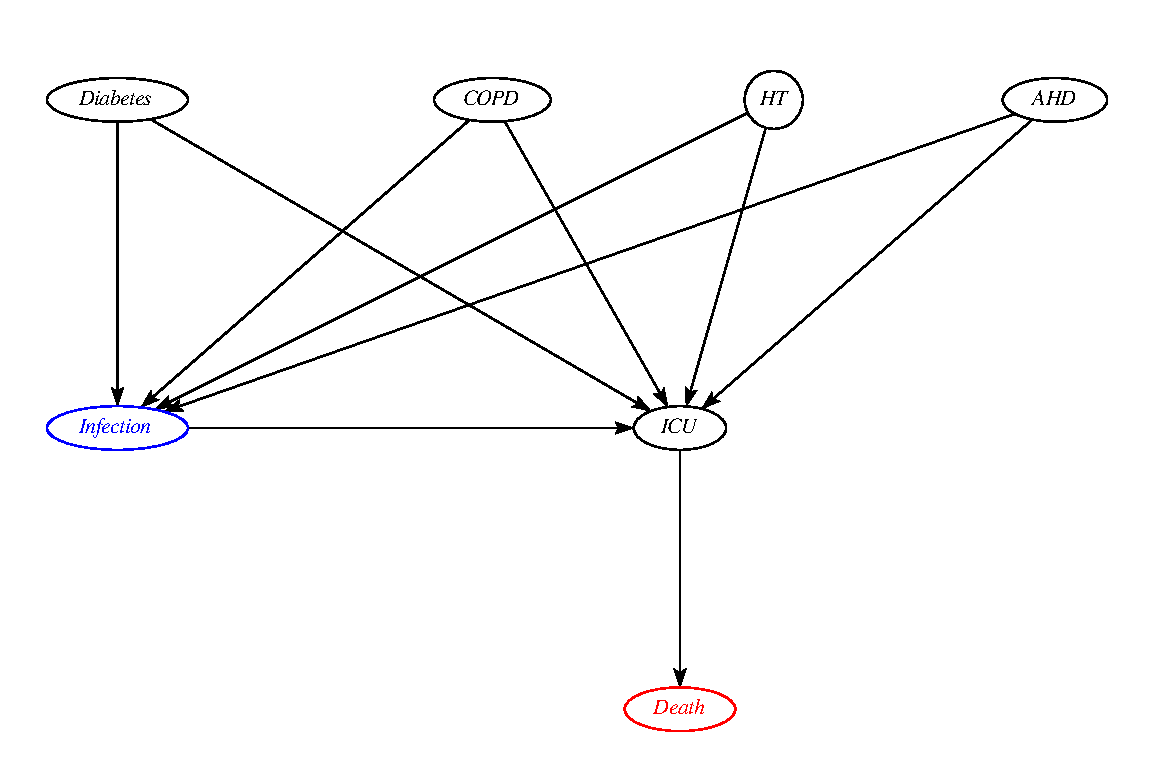
\includegraphics[width=0.6\textwidth]{figure1.pdf}
	\caption{Causal Graph $G$. $Infection$ is the treatment variable, and $Death$ is the outcome variable.}
	\label{figure1}
\end{figure}

\section{Derivation}

\begin{theorem}
	The causal effect of $Infection$ on $Death$ is identifiable from $P_{}\left(AHD,COPD,Death,Diabetes,HT,ICU,Infection\right)$ and is given by the formula
	\[ P_{Infection}\left(Death\right) = \sum_{AHD,COPD,Diabetes,HT}{P\left(Death \middle| Infection,AHD,COPD,Diabetes,HT\right)P\left(AHD,COPD,Diabetes,HT\right)} \]
\end{theorem}

\begin{proof}
	\begin{shiftedflalign}
		& P_{Infection}\left(Death\right) & \label{eq1} \\
		&= \sum_{AHD,COPD,Diabetes,HT,ICU}{P_{Infection}\left(AHD,COPD,Death,Diabetes,HT,ICU\right)} \label{eq2} \\
		&= \sum_{AHD,COPD,Diabetes,HT,ICU}{P_{COPD,Death,Diabetes,HT,ICU,Infection}\left(AHD\right)P_{AHD,Death,Diabetes,HT,ICU,Infection}\left(COPD\right)P_{AHD,COPD,Death,HT,ICU,Infection}\left(Diabetes\right)P_{AHD,COPD,Death,Diabetes,ICU,Infection}\left(HT\right)P_{AHD,COPD,Death,Diabetes,HT,Infection}\left(ICU\right)P_{AHD,COPD,Diabetes,HT,ICU,Infection}\left(Death\right)} \label{eq3}
	\end{shiftedflalign}
	Eq. (\ref{eq2}) follows from summing over $\left\{ AHD,COPD,Diabetes,HT,ICU \right\}$ and Eq. (\ref{eq3})  from C-component factorization. \\\\
	\textbf{Task 1: Compute $P_{COPD,Death,Diabetes,HT,ICU,Infection}\left(AHD\right)$} 
	\begin{shiftedflalign}
		& P_{COPD,Death,Diabetes,HT,ICU,Infection}\left(AHD\right) & \label{eq4} \\
		&= P_{}\left(AHD\right) \label{eq5}
	\end{shiftedflalign}
	Eq. (\ref{eq5}) follows from the third rule of do-calculus with the independence $\left(COPD,Death,Diabetes,HT,ICU,Infection \perp AHD\right)_{G_{\overline{COPD,Death,Diabetes,HT,ICU,Infection}}}$ (refer to Fig. \ref{figure2}). \\\\
	\textbf{Task 2: Compute $P_{AHD,Death,Diabetes,HT,ICU,Infection}\left(COPD\right)$} 
	\begin{shiftedflalign}
		& P_{AHD,Death,Diabetes,HT,ICU,Infection}\left(COPD\right) & \label{eq6} \\
		&= P_{}\left(COPD\right) \label{eq7}
	\end{shiftedflalign}
	Eq. (\ref{eq7}) follows from the third rule of do-calculus with the independence $\left(AHD,Death,Diabetes,HT,ICU,Infection \perp COPD\right)_{G_{\overline{AHD,Death,Diabetes,HT,ICU,Infection}}}$ (refer to Fig. \ref{figure2}). \\\\
	\textbf{Task 3: Compute $P_{AHD,COPD,Death,HT,ICU,Infection}\left(Diabetes\right)$} 
	\begin{shiftedflalign}
		& P_{AHD,COPD,Death,HT,ICU,Infection}\left(Diabetes\right) & \label{eq8} \\
		&= P_{}\left(Diabetes\right) \label{eq9}
	\end{shiftedflalign}
	Eq. (\ref{eq9}) follows from the third rule of do-calculus with the independence $\left(AHD,COPD,Death,HT,ICU,Infection \perp Diabetes\right)_{G_{\overline{AHD,COPD,Death,HT,ICU,Infection}}}$ (refer to Fig. \ref{figure2}). \\\\
	\textbf{Task 4: Compute $P_{AHD,COPD,Death,Diabetes,ICU,Infection}\left(HT\right)$} 
	\begin{shiftedflalign}
		& P_{AHD,COPD,Death,Diabetes,ICU,Infection}\left(HT\right) & \label{eq10} \\
		&= P_{}\left(HT\right) \label{eq11}
	\end{shiftedflalign}
	Eq. (\ref{eq11}) follows from the third rule of do-calculus with the independence $\left(AHD,COPD,Death,Diabetes,ICU,Infection \perp HT\right)_{G_{\overline{AHD,COPD,Death,Diabetes,ICU,Infection}}}$ (refer to Fig. \ref{figure2}). \\\\
	\textbf{Task 5: Compute $P_{AHD,COPD,Death,Diabetes,HT,Infection}\left(ICU\right)$} 
	\begin{shiftedflalign}
		& P_{AHD,COPD,Death,Diabetes,HT,Infection}\left(ICU\right) & \label{eq12} \\
		&= {{P_{AHD,COPD,Diabetes,HT,Infection}\left(ICU\right)}} \label{eq13} \\
		&= {{P_{}\left(ICU \middle| AHD,COPD,Diabetes,HT,Infection\right)}} \label{eq14}
	\end{shiftedflalign}
	Eq. (\ref{eq13}) follows from the third rule of do-calculus with the independence $\left(Death \perp ICU | AHD,COPD,Diabetes,HT,Infection\right)_{G_{\overline{AHD,COPD,Death,Diabetes,HT,Infection}}}$ (refer to Fig. \ref{figure3}).
	Eq. (\ref{eq14}) follows from the second rule of do-calculus with the independence $\left(AHD,COPD,Diabetes,HT,Infection \perp ICU\right)_{G_{\overline{}\underline{AHD,COPD,Diabetes,HT,Infection}}}$ (refer to Fig. \ref{figure4}). \\\\
	\textbf{Task 6: Compute $P_{AHD,COPD,Diabetes,HT,ICU,Infection}\left(Death\right)$} 
	\begin{shiftedflalign}
		& P_{AHD,COPD,Diabetes,HT,ICU,Infection}\left(Death\right) & \label{eq15} \\
		&= {{P_{}\left(Death \middle| AHD,COPD,Diabetes,HT,ICU,Infection\right)}} \label{eq16}
	\end{shiftedflalign}
	Eq. (\ref{eq16}) follows from the second rule of do-calculus with the independence $\left(AHD,COPD,Diabetes,HT,ICU,Infection \perp Death\right)_{G_{\overline{}\underline{AHD,COPD,Diabetes,HT,ICU,Infection}}}$ (refer to Fig. \ref{figure2}). \\\\
	Substituting Eq. (\ref{eq5}), Eq. (\ref{eq7}), Eq. (\ref{eq9}), Eq. (\ref{eq11}), Eq. (\ref{eq14}), and Eq. (\ref{eq16}) back into Eq. (\ref{eq3}), we get
	\begin{flalign}
		P_{Infection}\left(Death\right) = \sum_{AHD,COPD,Diabetes,HT}{P\left(Death \middle| Infection,AHD,COPD,Diabetes,HT\right)P\left(AHD,COPD,Diabetes,HT\right)} \label{eq17}
	\end{flalign}
\end{proof}

\section{Figures}

The subgraphs used in the derivation of the causal effect of $Infection$ on $Death$ are as follows:

\begin{figure}[H]
	\centering
	\includegraphics[width=0.6\textwidth]{figure2.pdf}
	\caption{Causal Graph $G_{\overline{COPD,Death,Diabetes,HT,ICU,Infection}}, G_{\overline{AHD,Death,Diabetes,HT,ICU,Infection}}, G_{\overline{AHD,COPD,Death,HT,ICU,Infection}}, G_{\overline{AHD,COPD,Death,Diabetes,ICU,Infection}}, G_{\overline{}\underline{AHD,COPD,Diabetes,HT,ICU,Infection}}$.}
	\label{figure2}
\end{figure}

\begin{figure}[H]
	\centering
	\includegraphics[width=0.6\textwidth]{figure3.pdf}
	\caption{Causal Graph $G_{\overline{AHD,COPD,Death,Diabetes,HT,Infection}}$.}
	\label{figure3}
\end{figure}

\begin{figure}[H]
	\centering
	\includegraphics[width=0.6\textwidth]{figure4.pdf}
	\caption{Causal Graph $G_{\overline{}\underline{AHD,COPD,Diabetes,HT,Infection}}$.}
	\label{figure4}
\end{figure}

\end{document}